\chapter{Design}

\section*{Introduction}
\addcontentsline{toc}{section}{Introduction}

This chapter presents the design of Football OS and answers how the platform is
organized and how the main processes are implemented. It focuses on the global
architecture, backend module design, data design, processing design, and
security and authorization design.

\section{Global Architecture Design}

\subsection{Architectural Style and Decision Analysis}

Football OS adopts a microservices-oriented architecture organized inside a
monorepo. The system is not implemented as a single monolithic backend: the
API Gateway, Governance Service, and Workspace Service are separated as
distinct backend applications with their own responsibilities, runtime
configuration, and persistence concerns. The monorepo structure was kept to
simplify development, dependency management, and Shared SDK evolution during
the internship.

This choice provides a compromise between a simple monolith and a fully
distributed multi-repository microservices ecosystem. A monolith would have
reduced deployment complexity but would have mixed governance, workspace
operations, authorization, and document workflows inside one application. A
fully independent multi-repository microservices organization would have
increased operational overhead, CI/CD complexity, and version-management cost.
The selected architecture keeps clear service boundaries while remaining
manageable for a small-team academic project.

Classic SOA is retained in this report only as a comparison baseline, while the
implemented backend aligns with a microservices-oriented monorepo model
\cite{soa-erl,microservices-newman}. Backend service internals still follow
Onion/Clean Architecture layering to keep domain logic isolated from technical
adapters \cite{clean-arch}.

\begin{table}[ht]
\centering
\caption{Architecture decision matrix}
\label{tab:architecture-decision-matrix}
\small
\setlength{\tabcolsep}{3pt}
\renewcommand{\arraystretch}{1.08}
\begin{tabularx}{\textwidth}{|L{3.0cm}|C{1.8cm}|C{1.8cm}|C{2.5cm}|Y|}
\hline
\textbf{Criterion} & \textbf{Monolith} & \textbf{Classic SOA} & \makecell[c]{\textbf{Multi-repository}\\\textbf{Microservices}} & \makecell[c]{\textbf{Selected}\\\textbf{Microservices Monorepo}} \\
\hline
Maintainability & Medium & Medium & High & High \\
\hline
\makecell[l]{Deployment\\complexity} & Low & Medium & High & Medium \\
\hline
Domain ownership & Low & Medium & High & High \\
\hline
Security isolation & Medium & Medium & High & High \\
\hline
\makecell[l]{Team-size\\suitability} & High (small team) & Medium & Low (small team) & High (small team) \\
\hline
Latency overhead & Low & Medium & High & Medium \\
\hline
\makecell[l]{Shared code\\management} & \makecell[c]{Simple but\\coupled} & Moderate & \makecell[c]{Difficult\\across repos} & \makecell[c]{Centralized\\and controlled} \\
\hline
\end{tabularx}
\normalsize
\end{table}

The selected option is therefore not a classic centralized SOA model, but a
microservices-oriented monorepo. Gateway owns edge enforcement, Governance owns
identity/canonical/policy/audit concerns, Workspace owns operational document,
event, profile, and notification workflows, and the Shared SDK reduces
duplicated integration code while preserving service-level separation.

\subsection{General Architecture}

The following diagram shows how the frontend communicates with the backend
through the Gateway, and how backend services rely on governance, workspace,
SDK, and supporting infrastructure.

\begin{figure}[ht]
    \centering
    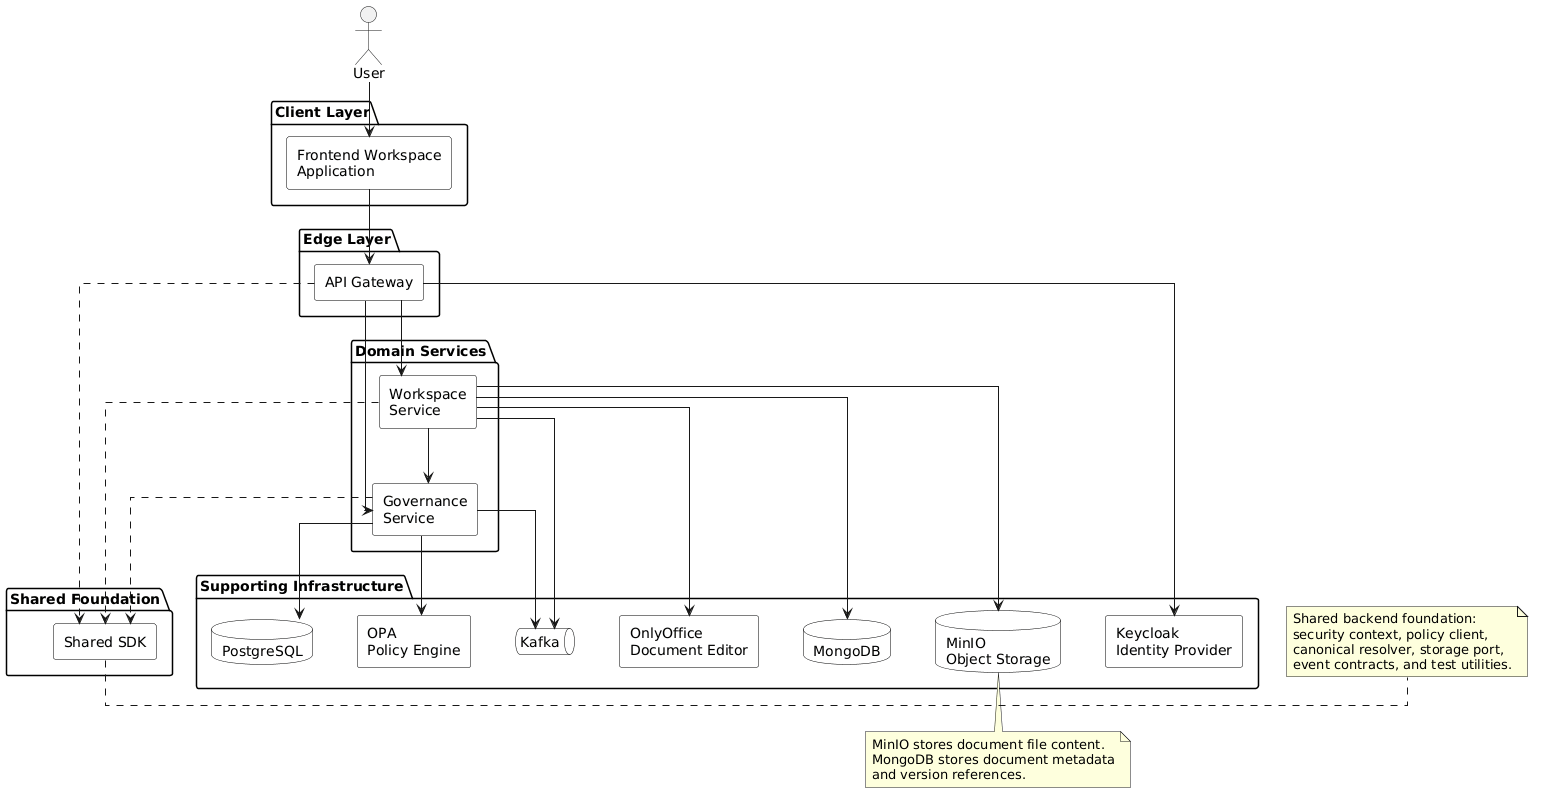
\includegraphics[width=0.95\textwidth]{images/architecture-logique.png}
    \caption{Global architecture of the Football OS platform}
    \label{fig:global-architecture}
\end{figure}

As shown in Figure~\ref{fig:global-architecture}, the frontend sends requests
to the API Gateway, which routes calls to Governance or Workspace. The SDK
provides shared abstractions, while infrastructure supports persistence,
messaging, policy evaluation, storage, and document editing. The asynchronous
communication design follows event-driven integration principles \cite{eda-fowler}.

\begin{table}[ht]
\centering
\caption{Default local entry points used during development}
\label{tab:local-entry-points}
\begin{tabular}{|p{4.5cm}|p{3cm}|p{6.5cm}|}
\hline
\textbf{Component} & \textbf{Port} & \textbf{Access role} \\
\hline
Workspace Frontend & 4200 & User web interface. \\
\hline
API Gateway & 8080 & Public backend entry point for frontend API calls. \\
\hline
Governance Service & 8081 & Internal/backend endpoint behind Gateway routing. \\
\hline
Workspace Service & 8082 & Internal/backend endpoint behind Gateway routing. \\
\hline
\end{tabular}
\end{table}

Table~\ref{tab:local-entry-points} clarifies that frontend API traffic goes
through the Gateway rather than directly to internal services.

\subsection{Main Components}

\begin{table}[ht]
\centering
\caption{Main components of the Football OS architecture}
\label{tab:main-components}
\small
\setlength{\tabcolsep}{4pt}
\renewcommand{\arraystretch}{1.10}
\begin{tabularx}{\textwidth}{|L{3.7cm}|Y|L{3.3cm}|}
\hline
\textbf{Component} & \textbf{Responsibility} & \textbf{Main Technology} \\
\hline
Frontend Workspace Application & User interface for workspace operations and platform access. & Angular + Tailwind CSS \\
\hline
API Gateway & Entry point of backend APIs; routes requests and enforces secure access flow. & Spring Boot (Gateway layer) \\
\hline
Governance Service & Manages users, roles, permissions, canonical players/teams, policy decisions, and audit tracking. & Spring Boot + PostgreSQL + OPA \\
\hline
Workspace Service & Manages documents, calendar/events, notifications, search, and player profile aggregation. & Spring Boot + MongoDB + MinIO \\
\hline
Shared SDK & Shared foundation/library used by backend services; provides reusable abstractions and common integration mechanisms. & Java multi-module SDK \\
\hline
Keycloak / Identity Provider & Authenticates users and provides identity context. & Keycloak (OIDC/JWKS) \\
\hline
OPA Policy Engine & Evaluates authorization rules for protected actions and resources. & Open Policy Agent \\
\hline
Kafka & Supports asynchronous event messaging and notification propagation. & Apache Kafka \\
\hline
PostgreSQL & Stores governance structured data such as actors, roles, players, teams, and audit logs. & PostgreSQL \\
\hline
MongoDB & Stores workspace aggregates and document metadata/version references, including documents, events, and notifications. & MongoDB \\
\hline
MinIO & Stores the actual document file content and file versions. & MinIO Object Storage \\
\hline
Redis & Supports gateway-level rate limiting and request throttling. & Redis \\
\hline
OnlyOffice & Enables online document viewing and editing workflows. & OnlyOffice Docs \\
\hline
\end{tabularx}
\normalsize
\end{table}

Table~\ref{tab:main-components} summarizes the main technical responsibilities
and technologies used by each architecture component.

\section{Backend Module Design}

\subsection{API Gateway}

The API Gateway is the backend entry point. It validates token context, applies
edge controls, and routes requests to Governance and Workspace without exposing
internal service addresses.

\subsection{Governance Service}

The Governance Service owns actor/role management, canonical players/teams,
policy decision support through OPA, and audit traceability data.

\subsection{Workspace Service}

The Workspace Service owns operational modules (documents, events,
notifications, search, and profile aggregation), persists workspace aggregates
in MongoDB, and integrates with Governance, MinIO, Kafka, and OnlyOffice.

\subsection{Shared SDK}

The Shared SDK is not a user-facing module. It is reused by backend services to
avoid duplicated technical plumbing. It provides shared security context,
policy client, canonical resolver, storage port abstraction, event contracts,
audit hooks, and test utilities.

\subsection{Service Boundary Summary}

\begin{table}[ht]
\centering
\caption{Service boundary summary}
\label{tab:module-responsibility}
\small
\setlength{\tabcolsep}{4pt}
\renewcommand{\arraystretch}{1.10}
\begin{tabularx}{\textwidth}{|L{2.8cm}|Y|L{2.2cm}|Y|}
\hline
\textbf{Service / Module} & \textbf{Ownership} & \textbf{Persistence} & \textbf{Main integrations} \\
\hline
API Gateway & Edge security, request enrichment, rate limiting, and routing to backend services. & No business DB & Keycloak JWKS, Redis, Governance Service, Workspace Service \\
\hline
Governance Service & Actors, roles, canonical players/teams, policy evaluation flow, and audit ownership. & PostgreSQL & OPA, Kafka, Keycloak, Shared SDK \\
\hline
Workspace Service & Documents, events, profiles, notifications, search, and OnlyOffice-related workflows. & MongoDB + MinIO & Governance policy/canonical APIs, Kafka, OnlyOffice \\
\hline
Shared SDK & Shared contracts and reusable adapters for security, policy, canonical, storage, events, and tests. & No business DB & Security, policy, canonical, storage, events, tests \\
\hline
\end{tabularx}
\normalsize
\end{table}
Table~\ref{tab:module-responsibility} consolidates the separation of
responsibilities across backend modules.

\subsection{API Summary}

Table~\ref{tab:api-summary} provides a compact overview of representative
endpoint families used by the platform.

\begin{table}[ht]
\centering
\caption{API endpoint family summary}
\label{tab:api-summary}
\small
\renewcommand{\arraystretch}{1.10}
\setlength{\tabcolsep}{4pt}
\begin{tabularx}{\textwidth}{|L{2.4cm}|L{3.8cm}|Y|}
\hline
\textbf{Module} & \textbf{Endpoint family} & \textbf{Purpose} \\
\hline
Workspace & \makecell[l]{\texttt{/api/v1/}\\\texttt{documents}} & Document upload, consultation, categorization, and lifecycle operations. \\
\hline
Workspace & \makecell[l]{\texttt{/api/v1/}\\\texttt{events}} & Event creation, consultation, update, and archive workflows. \\
\hline
Workspace & \makecell[l]{\texttt{/api/v1/}\\\texttt{profiles}} & Role-filtered player profile consultation and aggregation. \\
\hline
Workspace & \makecell[l]{\texttt{/api/v1/}\\\texttt{notifications}} & Notification generation, retrieval, and state updates. \\
\hline
Workspace & \makecell[l]{\texttt{/api/v1/}\\\texttt{search}} & Search across workspace resources with access filtering. \\
\hline
Workspace & \makecell[l]{\texttt{/api/v1/}\\\texttt{onlyoffice}} & Online document editor integration and callback-related actions. \\
\hline
Governance & \makecell[l]{\texttt{/api/v1/}\\\texttt{actors}} & Actor management and actor-role relationship management. \\
\hline
Governance & \makecell[l]{\texttt{/api/v1/}\\\texttt{players}} & Canonical player data operations and references. \\
\hline
Governance & \makecell[l]{\texttt{/api/v1/}\\\texttt{teams}} & Canonical team data operations and references. \\
\hline
Governance & \makecell[l]{\texttt{/api/v1/}\\\texttt{policy}} & Authorization decision endpoints for protected actions. \\
\hline
\end{tabularx}
\normalsize
\setlength{\tabcolsep}{6pt}
\end{table}

\section{Data Design}

\subsection{Main Data Models}

Football OS uses several services and storage technologies. For this reason,
the data model is presented by domain instead of using one large global class
diagram. Governance entities are persisted in PostgreSQL, workspace aggregates
in MongoDB, and binary document content in MinIO.

\subsection{Governance Relational Entities (PostgreSQL)}

\begin{table}[H]
\centering
\caption{Governance entities stored in PostgreSQL}
\label{tab:governance-postgresql}
\small
\setlength{\tabcolsep}{4pt}
\renewcommand{\arraystretch}{1.10}
\begin{tabularx}{\textwidth}{|L{2.5cm}|C{1.9cm}|Y|Y|}
\hline
\textbf{Entity} & \textbf{Storage} & \textbf{Main fields} & \textbf{Purpose} \\
\hline
Actor & PostgreSQL & id, identityRef, roleRefs, status & Represents platform actors and identity linkage. \\
\hline
Role & PostgreSQL & id, roleCode, permissions & Defines permission sets for authorization decisions. \\
\hline
Player & PostgreSQL & id, canonicalRef, names, teamRef & Maintains canonical player references used across modules. \\
\hline
Team & PostgreSQL & id, canonicalRef, name, metadata & Maintains canonical team references. \\
\hline
AuditLogEntry & PostgreSQL & id, actorRef, action, target, timestamp & Records traceable governance and access-related operations. \\
\hline
\end{tabularx}
\normalsize
\setlength{\tabcolsep}{6pt}
\end{table}
Table~\ref{tab:governance-postgresql} summarizes the governance entities and
their persistence responsibilities.

\subsection{Workspace Collections (MongoDB)}

\begin{table}[H]
\centering
\caption{Workspace collections stored in MongoDB}
\label{tab:workspace-mongodb}
\small
\renewcommand{\arraystretch}{1.10}
\setlength{\tabcolsep}{4pt}
\begin{tabularx}{\textwidth}{|L{2.9cm}|L{3.0cm}|Y|Y|}
\hline
\textbf{Collection} & \textbf{Stores} & \textbf{Main fields} & \textbf{Purpose} \\
\hline
\makecell[l]{\texttt{workspace\_}\\\texttt{documents}} & Document metadata and versions & id, category, state, versionRefs, ownerRef & Supports document lifecycle and lookup. \\
\hline
\makecell[l]{\texttt{workspace\_}\\\texttt{events}} & Events and linked operational items & id, type, schedule, attendees, tasks, requiredDocuments & Supports event planning and tracking flows. \\
\hline
\makecell[l]{\texttt{workspace\_}\\\texttt{notifications}} & User notification entries & id, userRef, message, state, createdAt & Supports notification delivery and read-state tracking. \\
\hline
\end{tabularx}
\normalsize
\end{table}
Table~\ref{tab:workspace-mongodb} summarizes the workspace collections used by
operational modules.

\subsection{Indexing and Consistency Strategy}
\label{sec:indexing-consistency-strategy}

Since Football OS separates governance data, workspace aggregates, and binary
files across different storage systems, data access must rely on clear
references and targeted indexes rather than cross-database foreign keys.

\begin{table}[H]
\centering
\caption{Indexing and reference strategy}
\label{tab:indexing-reference-strategy}
\small
\setlength{\tabcolsep}{4pt}
\renewcommand{\arraystretch}{1.10}
\begin{tabularx}{\textwidth}{|L{3.3cm}|L{4.2cm}|Y|}
\hline
\textbf{Storage} & \textbf{Index / Reference} & \textbf{Purpose} \\
\hline
\makecell[l]{PostgreSQL\\Actor} & identityRef, roleRefs & Fast actor lookup and role resolution. \\
\hline
\makecell[l]{PostgreSQL\\Player} & canonicalRef, teamRef & Player and team reference lookup. \\
\hline
\makecell[l]{MongoDB\\\texttt{workspace\_docu-}\\\texttt{ments}} & category, state, ownerRef & Document filtering by visibility, ownership, and lifecycle state. \\
\hline
\makecell[l]{MongoDB\\\texttt{workspace\_-}\\\texttt{events}} & \texttt{schedule.startDate}, \texttt{attendees.actorRef} & Calendar listing and attendee-based event lookup. \\
\hline
\makecell[l]{MongoDB\\\texttt{workspace\_notifi-}\\\texttt{cations}} & userRef, state, createdAt & Inbox retrieval and unread notification queries. \\
\hline
\makecell[l]{MinIO\\object keys} & bucket, objectKey, version reference & Binary file retrieval without storing large files directly in MongoDB or PostgreSQL. \\
\hline
\end{tabularx}
\normalsize
\setlength{\tabcolsep}{6pt}
\end{table}

Cross-service references are stored as identifiers rather than relational
foreign keys across databases. Governance remains the source of truth for
actors, roles, players, and teams, while Workspace stores references to these
canonical entities. When canonical data is required, Workspace resolves it
through Governance and SDK integration instead of duplicating governance state.
This approach reduces coupling between databases, but it also requires careful
handling of unavailable references and eventual consistency between services.

\subsection{Governance Service Design}

\noindent The Governance Service acts as the control plane of Football OS. It
centralizes identity management, canonical football entities, authorization
decisions, signal processing, and audit traceability. The first governance
diagram in this section is intentionally a package-level dependency view, not a
class-level model. It provides a global structural perspective before zooming
into selected internal packages.

\subsubsection{Governance Service Package Dependency Diagram}

\noindent The governance codebase is organized into feature packages:
\texttt{canonical}, \texttt{identity}, \texttt{policy}, \texttt{signal}, and
\texttt{config}. Inside \texttt{canonical}, \texttt{identity},
\texttt{policy}, and \texttt{signal}, the structure follows layered packages:
\texttt{api}, \texttt{application}, \texttt{domain} (where applicable), and
\texttt{infrastructure}. The dependency direction remains explicit:
\texttt{api} depends on \texttt{application}; \texttt{application} coordinates
domain rules and infrastructure adapters; and \texttt{infrastructure}
integrates persistence and external systems. The \texttt{config} package wires
cross-cutting concerns such as security, exception handling, policy
configuration, and signal pipeline configuration. Dashed arrows represent UML
dependency relationships between packages.

\clearpage
\begin{figure}[H]
\centering
\makebox[\textwidth][c]{%
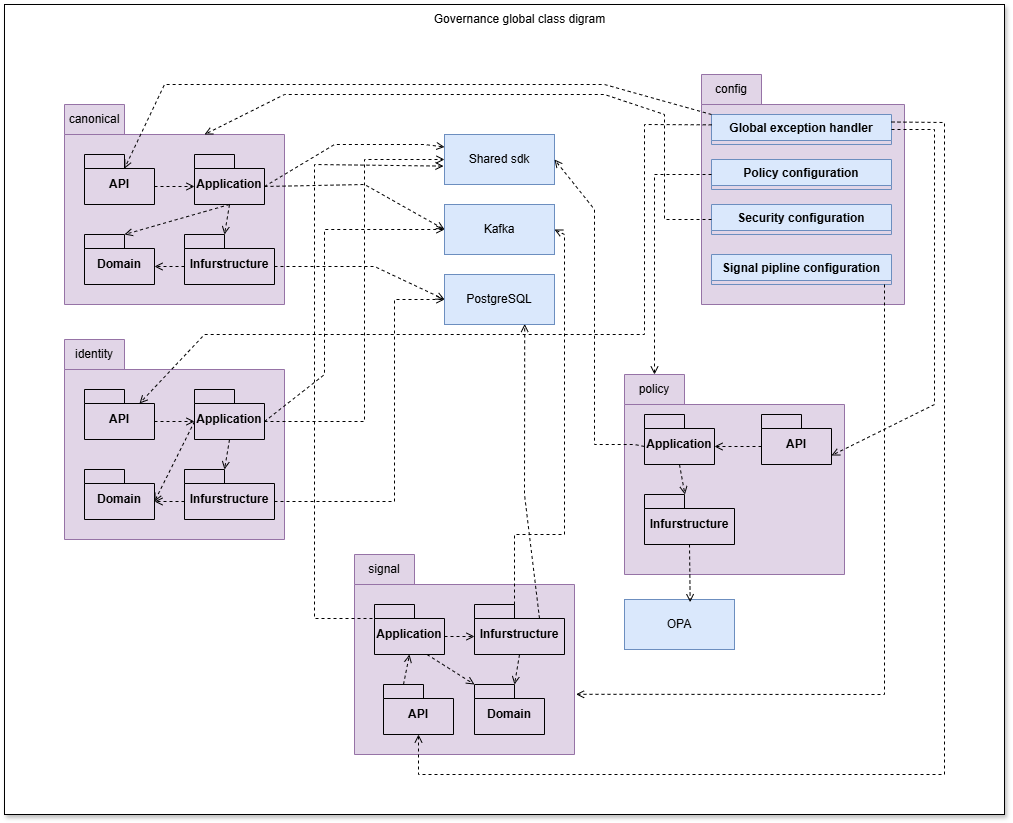
\includegraphics[width=1.20\textwidth,height=0.88\textheight,keepaspectratio]{images/classdig/gov-dig.png}%
}
\caption{Governance service package dependency diagram}
\label{fig:governance-package-diagram}
\end{figure}

\subsubsection{Policy Package Class Diagram}

\noindent The policy package is detailed because it represents the
authorization decision flow implemented in the backend. The API layer receives
policy evaluation requests, the application layer builds and evaluates policy
context, and the infrastructure layer communicates with OPA for decision
execution. Shared SDK contracts standardize request and response models across
services. This diagram emphasizes that authorization is delegated to the
governance policy mechanism rather than enforced only in frontend logic.

\clearpage
\begin{figure}[H]
\centering
\makebox[\textwidth][c]{%
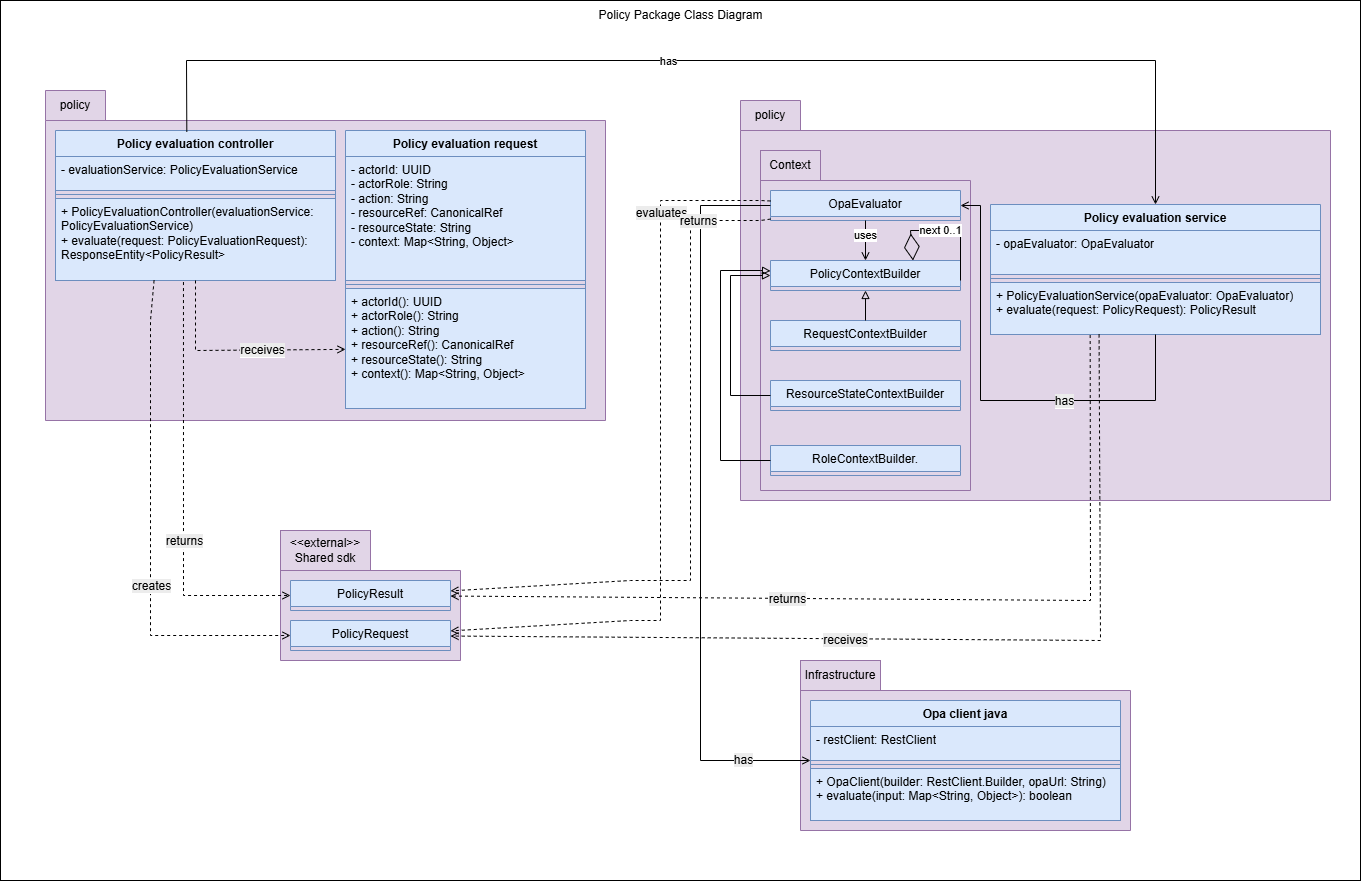
\includegraphics[width=1.20\textwidth,height=0.88\textheight,keepaspectratio]{images/classdig/policy.drawio.png}%
}
\caption{Policy package class diagram}
\label{fig:policy-class-diagram}
\end{figure}

\subsubsection{Signal Package Class Diagram}

\noindent The signal package is detailed because it captures event intake,
processing, routing, notification fan-out, and audit/event propagation. Its
internal organization follows a processing pipeline (chain) structure and
integrates with Kafka messaging and audit persistence. This view complements
the package dependency diagram by exposing the internal signal-processing
collaboration.

\clearpage
\begin{figure}[H]
\centering
\makebox[\textwidth][c]{%
\IfFileExists{images/classdig/signal.drawio.png}{%
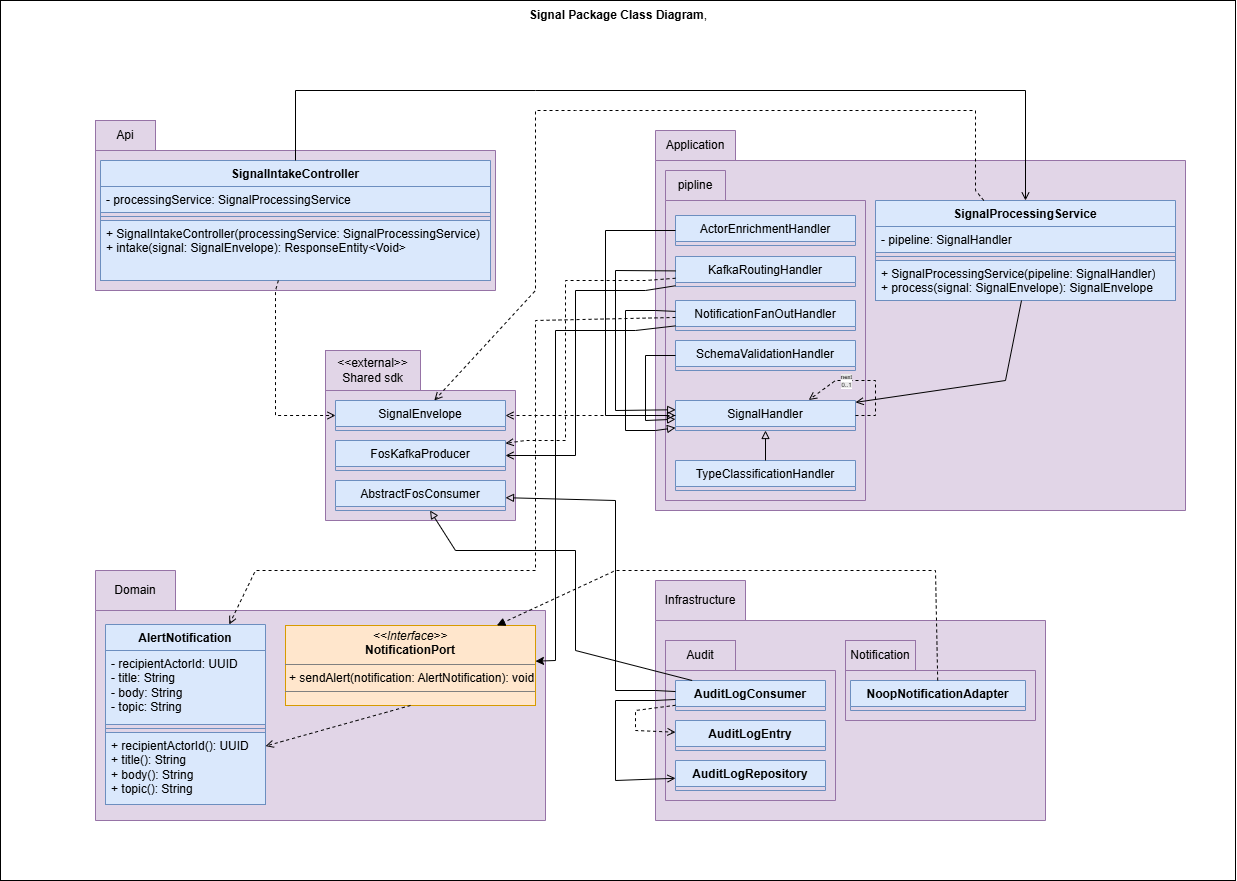
\includegraphics[width=1.20\textwidth,height=0.88\textheight,keepaspectratio]{images/classdig/signal.drawio.png}%
}{%
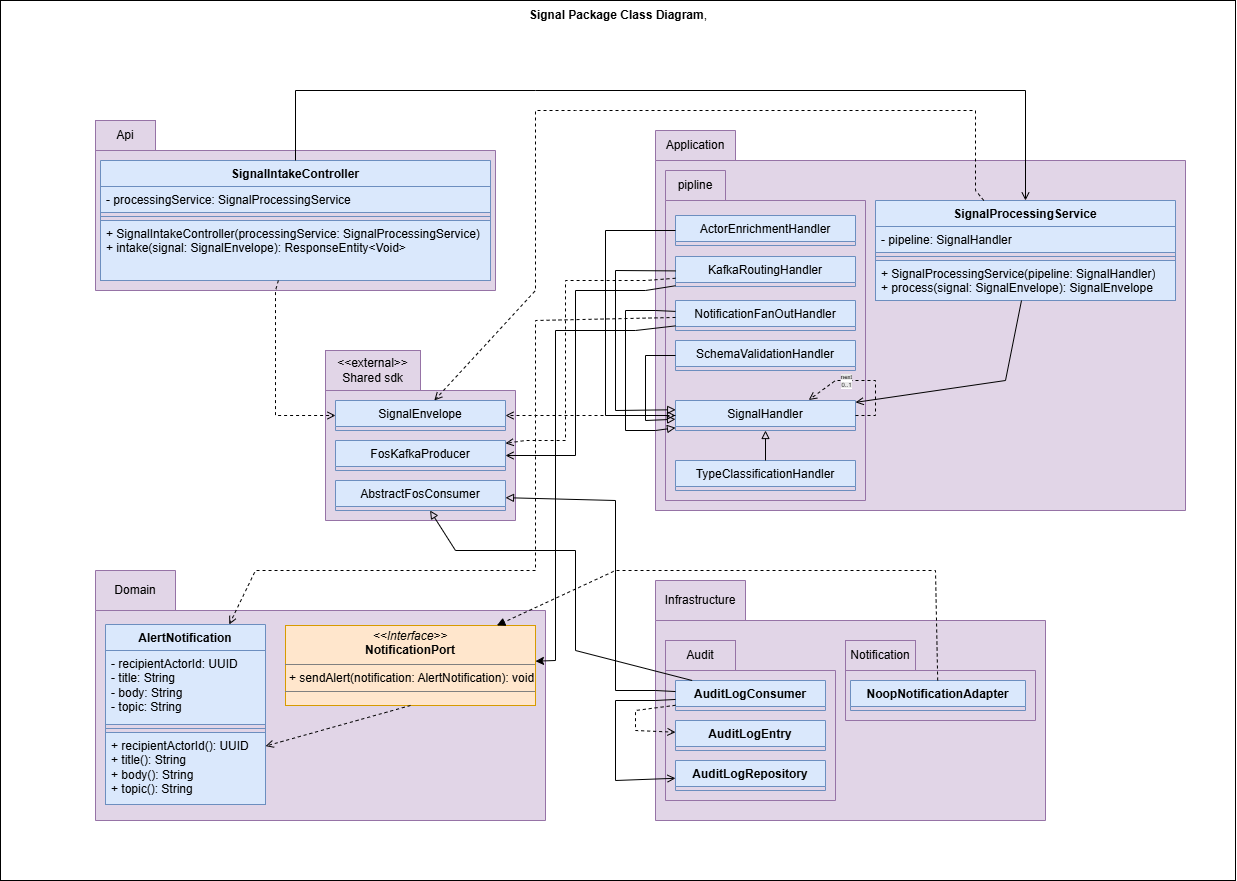
\includegraphics[width=1.20\textwidth,height=0.88\textheight,keepaspectratio]{images/classdig/signal-class-diagram.png}%
}%
}
\caption{Signal package class diagram}
\label{fig:signal-class-diagram}
\end{figure}

\subsubsection{Identity Package Class Diagram}

\noindent The identity package is detailed because it manages platform actors,
actor roles, lifecycle operations, and identity synchronization. It links
authentication identity context with governance-level actor representation.
The diagram focuses on the most relevant identity classes and relationships
rather than listing every technical file.

\clearpage
\begin{figure}[H]
\centering
\makebox[\textwidth][c]{%
\IfFileExists{images/classdig/identity-class-diagram.png}{%
\includegraphics[width=1.20\textwidth,height=0.88\textheight,keepaspectratio]{images/classdig/identity-class-diagram.png}%
}{%
\fbox{\begin{minipage}[c][0.22\textheight][c]{0.82\textwidth}\centering
Identity class diagram image missing:\\
\texttt{images/classdig/identity-class-diagram.png}
\end{minipage}}%
}%
}
\caption{Identity package class diagram}
\label{fig:identity-class-diagram}
\end{figure}

\noindent The following diagrams shift from governance control-plane internals
to workspace-side data structures, specifically document management and
calendar/event management.

\subsection{Document Management Class Diagram}

\noindent This diagram presents how documents are modeled through metadata,
version history, and storage links. It separates business metadata from file
content kept in object storage.

Figure~\ref{fig:document-class-diagram} highlights that WorkspaceDocument is
the main record, while DocumentVersion stores each file revision with bucket
and object-key references. DocumentCategory and DocumentState structure
classification and lifecycle control.

\clearpage
\begin{figure}[H]
\centering
\makebox[\textwidth][c]{%
\IfFileExists{images/classdig/document-class-dig.png}{%

\includegraphics[width=1.24\textwidth,height=0.92\textheight,keepaspectratio]{images/classdig/document-class-dig.png}%
}{%
\fbox{\begin{minipage}[c][0.24\textheight][c]{0.84\textwidth}\centering
Document class diagram image missing:\\
\texttt{images/classdig/document-class-dig.png}
\end{minipage}}%
}%
}
\caption{Document management class diagram}
\label{fig:document-class-diagram}
\end{figure}

\subsection{Calendar and Event Class Diagram}

\noindent This diagram explains how workspace events are modeled, including
attendees, required documents, and staff tasks linked to each event.

Figure~\ref{fig:event-class-diagram} shows that WorkspaceEvent stores core
event information (title, type, schedule, location, and description), while
AttendeeRef, RequiredDocument, and TaskAssignment capture participation and
operational follow-up. EventType and EventState define classification and
lifecycle, and delete actions are handled as archive operations.

\clearpage
\begin{figure}[p]
\centering
\makebox[\textwidth][c]{%
  \IfFileExists{images/classdig/calander-event-class-dig.png}{%
  
\includegraphics[width=0.96\textheight,height=1.36\textwidth,keepaspectratio,angle=-90]{images/classdig/calander-event-class-dig.png}%
  }{%
  \fbox{\begin{minipage}[c][0.24\textheight][c]{0.84\textwidth}\centering
  Calendar/event class diagram image missing:\\
  \texttt{images/classdig/calander-event-class-dig.png}
  \end{minipage}}%
  }%
}
\caption{Calendar and event class diagram}
\label{fig:event-class-diagram}
\end{figure}
\clearpage

\subsection{Storage Mapping}

\begin{table}[ht]
\centering
\caption{Storage mapping for Football OS}
\label{tab:storage-mapping}
\begin{tabular}{|p{4.5cm}|p{9.5cm}|}
\hline
\textbf{Storage Element} & \textbf{Used For} \\
\hline
PostgreSQL & Governance structured data such as actors, roles, players, teams, and audit logs \\
\hline
MongoDB & Workspace aggregates such as documents, document versions, events, and notifications \\
\hline
MinIO & Actual uploaded files and edited document versions \\
\hline
Keycloak & Authentication and identity provider data \\
\hline
OPA & Authorization policy rules \\
\hline
Kafka & Asynchronous events and operational signals between components \\
\hline
Redis & Gateway rate limiting and request-throttling state \\
\hline
\end{tabular}
\end{table}

Table~\ref{tab:storage-mapping} summarizes storage responsibilities in Football
OS, while Subsection~\ref{sec:indexing-consistency-strategy} explains
cross-service references and consistency handling across these stores.

The player profile is not represented as a separate class diagram in the main
chapter because it is built by aggregating canonical player data, workspace
documents, policy decisions, and storage download links. It is therefore
explained in the processing design section.

\section{Processing Design}

This section analyzes four core processing flows used by the platform.

\subsection{Authentication Process Flow}

This flow covers authentication and token-based access across the user,
frontend, Gateway, identity provider, and backend services.

\begin{figure}[ht]
    \centering
    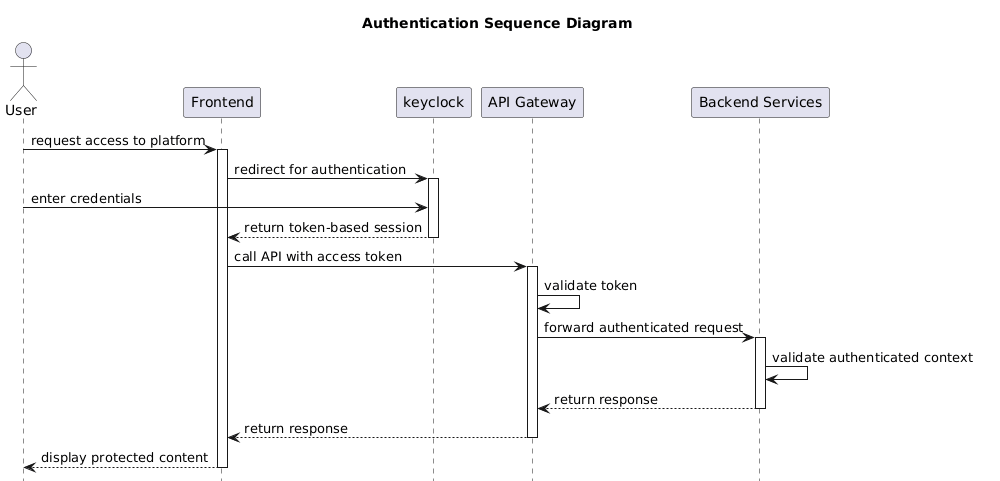
\includegraphics[width=\textwidth,height=0.52\textheight,keepaspectratio]{images/sequencedig/auth-seq.png}
    \caption{Authentication sequence diagram}
    \label{fig:authentication-sequence}
\end{figure}

Figure~\ref{fig:authentication-sequence} highlights the security boundary
created by the API Gateway. The frontend never calls internal services
directly; instead, authenticated requests pass through the Gateway, where token
validation and actor-context propagation are centralized. This flow reduces
duplicated authentication logic in downstream services while keeping protected
backend APIs behind a single controlled entry point.

\noindent The authentication flow is executed through the following steps:
\begin{enumerate}
    \item The user requests access from the frontend.
    \item The frontend redirects the user to the identity provider.
    \item The user authenticates and receives a token-based session.
    \item The frontend calls backend APIs through the Gateway with the token.
    \item Backend services validate the authenticated context before processing.
\end{enumerate}
Exception / alternative flow: if the token is invalid, expired, or missing, the
request is rejected and access is denied.

\subsection{Document Management Flow}

This flow covers document upload, access, and online editing.

\begin{figure}[ht]
    \centering
    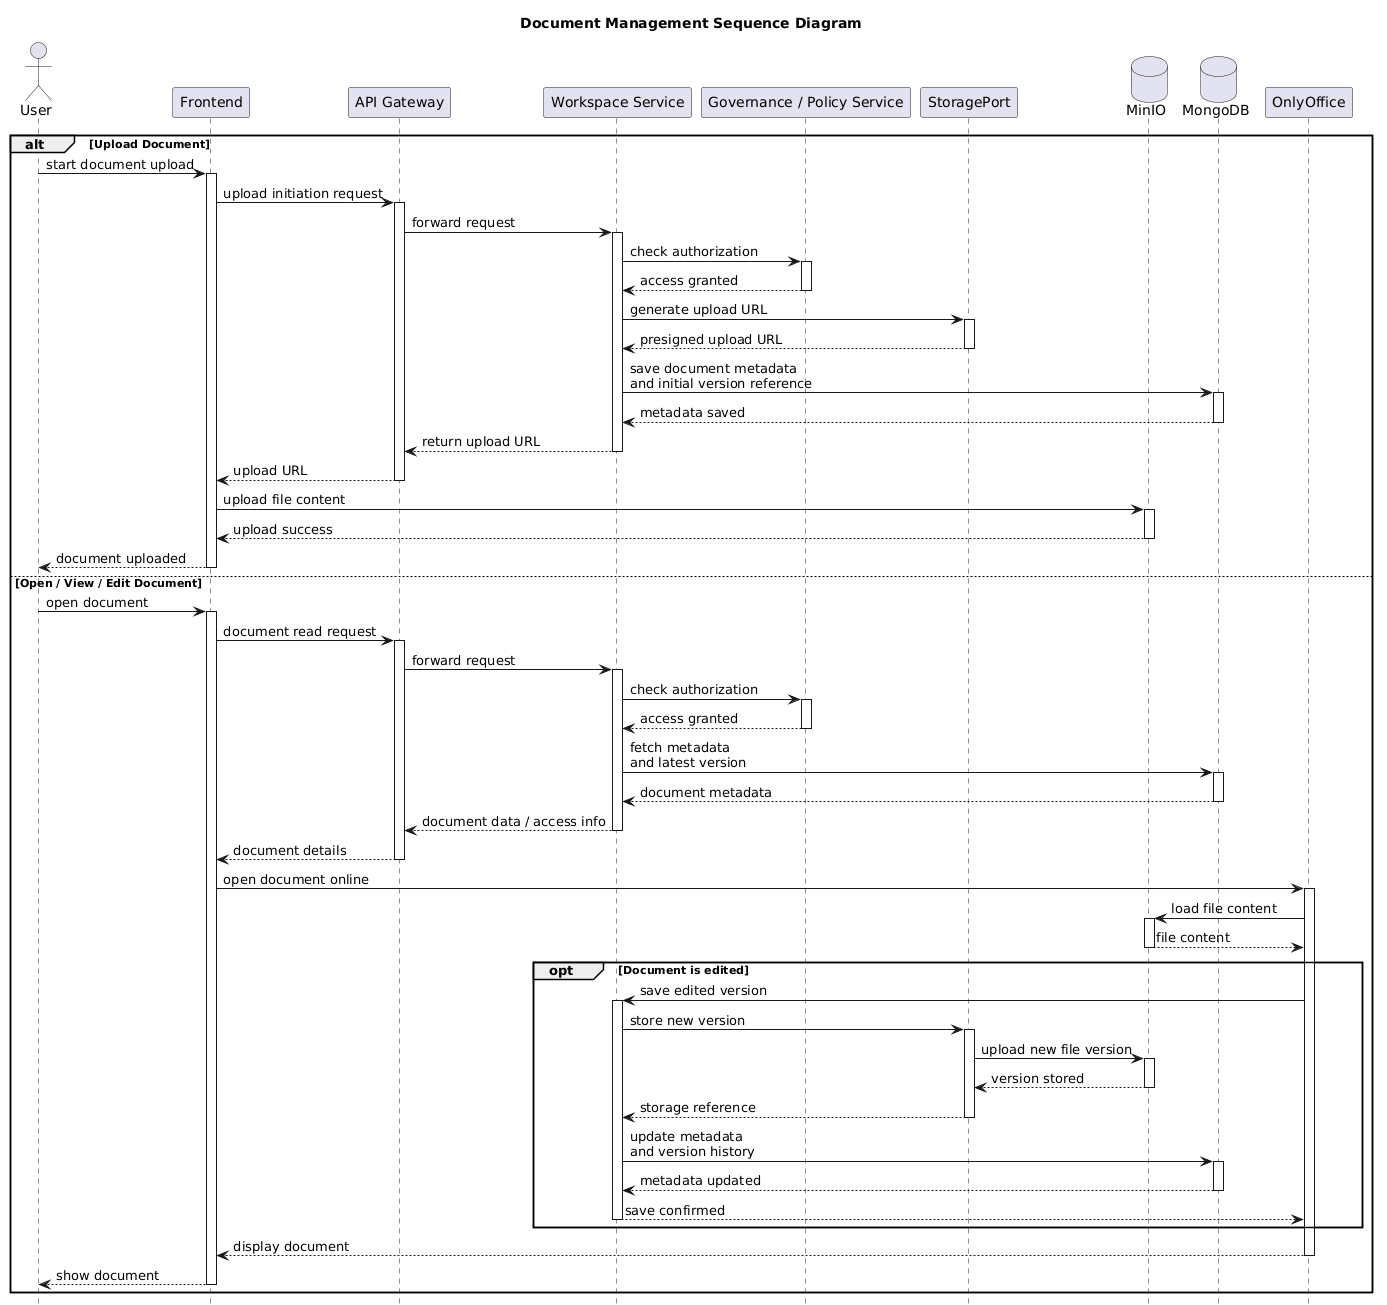
\includegraphics[width=0.95\textwidth]{images/sequencedig/doc-mangment-seq.png}
    \caption{Document management sequence diagram}
    \label{fig:document-management-sequence}
\end{figure}

Figure~\ref{fig:document-management-sequence} highlights the critical path of
document management. Authorization is performed before storage or editor access
is generated, which prevents unauthorized users from obtaining file URLs or
editor configurations. The separation between MongoDB metadata and MinIO binary
storage also preserves version history without storing large files directly
inside the database.

The flow executes through the following steps:
\begin{enumerate}
    \item The user uploads or opens a document through the frontend and Gateway.
    \item Workspace verifies authorization through Governance/Policy.
    \item For upload, Workspace generates a storage URL and the file is stored in MinIO.
    \item Metadata and version information are stored in MongoDB.
    \item Online viewing/editing is handled through OnlyOffice, and edited content is saved as a new version.
\end{enumerate}
Exception / alternative flow: if policy denies the action, no storage URL is
generated and the document operation is refused.

\subsection{Calendar and Event Management Flow}

This flow covers event creation, update, archival, and notification generation.

\begin{figure}[ht]
    \centering
    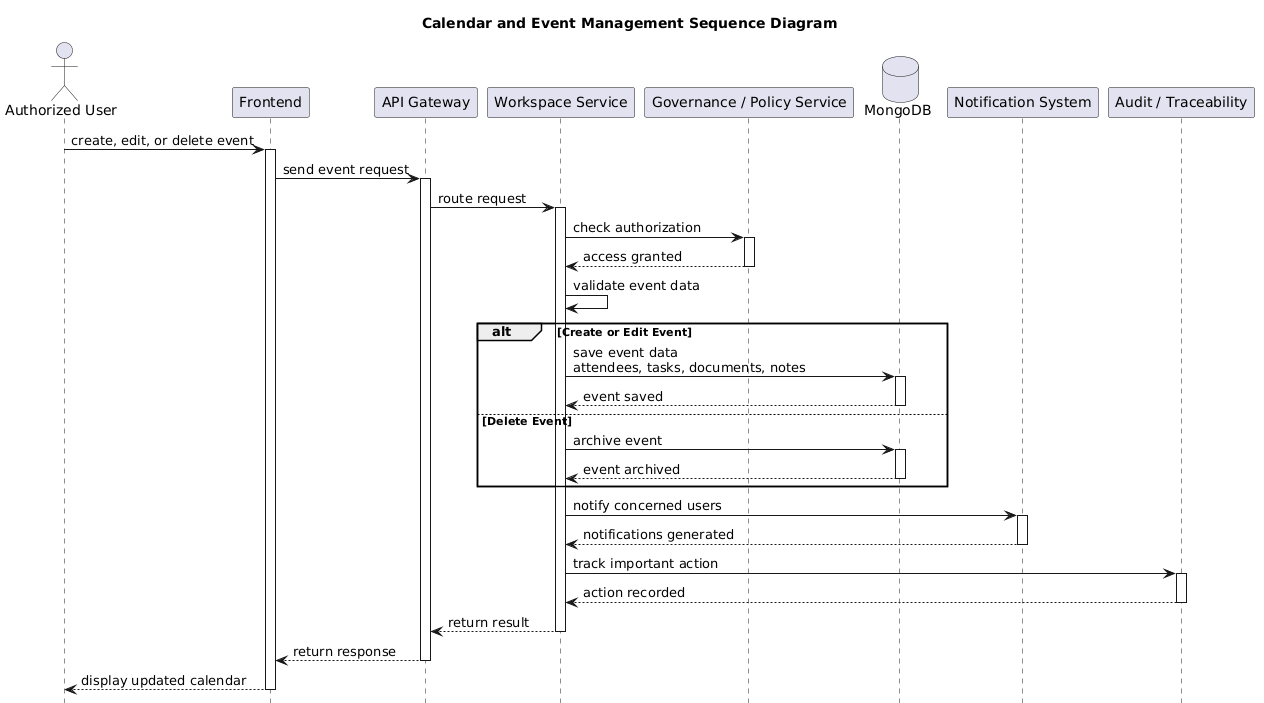
\includegraphics[width=0.95\textwidth]{images/sequencedig/calnder-seq.png}
    \caption{Calendar and event management sequence diagram}
    \label{fig:calendar-event-sequence}
\end{figure}

Figure~\ref{fig:calendar-event-sequence} emphasizes that event operations are
not limited to simple calendar updates. Each accepted action combines
authorization, data validation, persistence, notification generation, and
traceability. This flow is important because event changes may affect several
staff members and must therefore remain consistent, visible to concerned users,
and auditable.

The flow executes through the following steps:
\begin{enumerate}
    \item An authorized user creates, updates, or archives an event through the Gateway.
    \item Workspace validates data and verifies authorization.
    \item Event aggregates (including attendees, tasks, and required documents) are stored in MongoDB.
    \item Notifications are generated for concerned users.
    \item Important actions are tracked for traceability.
\end{enumerate}
Exception / alternative flow: if the user is not authorized, the event is not
created, modified, or archived.

In this design, delete operations are implemented as archive actions rather
than hard deletion.

\subsection{Player Profile Consultation Flow}

This flow covers how the platform builds a secured player profile.

\begin{figure}[ht]
    \centering
    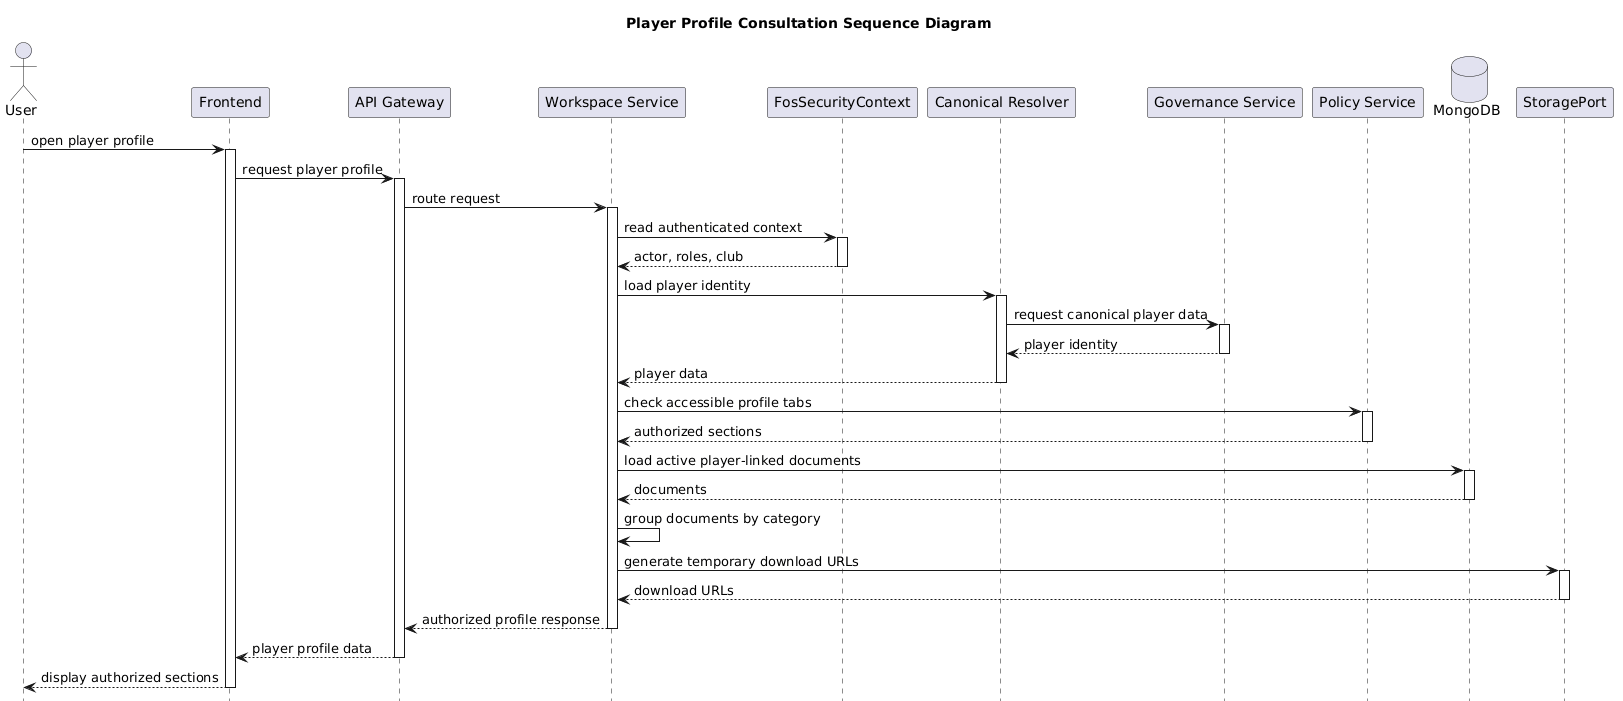
\includegraphics[width=0.95\textwidth]{images/sequencedig/player profile seq.png}
    \caption{Player profile consultation sequence diagram}
    \label{fig:player-profile-sequence}
\end{figure}

Figure~\ref{fig:player-profile-sequence} shows that player-profile consultation
is a filtered aggregation process rather than a direct database read. The
Workspace Service combines canonical player identity, workspace-linked
documents, storage references, and policy decisions before returning the
response. This protects sensitive sections, especially medical information, by
omitting unauthorized tabs and documents before the data reaches the frontend.

The flow executes through the following steps:
\begin{enumerate}
    \item The user requests a player profile through the frontend and Gateway.
    \item Workspace reads authenticated context and resolves canonical player identity.
    \item Workspace evaluates tab and section permissions through policy checks.
    \item Authorized player-linked documents are loaded and grouped by category.
    \item The response returns only permitted sections with temporary download links when needed.
\end{enumerate}
Exception / alternative flow: if policy denies sensitive sections, restricted
tabs are hidden and related data is omitted from the response.

\section{Security and Authorization Design}

Football OS combines identity-provider authentication, gateway-level token
validation, policy-based authorization, and backend-side access checks. The
security model is designed so that the frontend improves usability but does not
become the final enforcement point for protected resources
\cite{keycloak-doc,oauth2-rfc6749,oidc-core,rbac-sandhu,opa-doc}.

\subsection{Security Implementation Details}

\begin{table}[!htbp]
\centering
\caption{Security implementation choices}
\label{tab:security-implementation-choices}
\footnotesize
\setlength{\tabcolsep}{4pt}
\renewcommand{\arraystretch}{1.14}
\begin{tabularx}{\textwidth}{|L{3.2cm}|Y|}
\hline
\textbf{Security concern} & \textbf{Implementation choice} \\
\hline
Authentication & Keycloak with OIDC and JWT-based access tokens. \\
\hline
Token validation & API Gateway validates access tokens using Keycloak JWKS through the resource-server security configuration. \\
\hline
Session model & Backend services remain stateless and rely on token-based authentication context. \\
\hline
Token propagation & The frontend sends a bearer token to the Gateway; the Gateway enriches/forwards actor context to downstream services. \\
\hline
Authorization & Workspace calls the Governance policy endpoint, which relies on OPA-backed decisions. \\
\hline
Rate limiting & Gateway-level Redis-backed rate limiting protects backend entry points from excessive requests. \\
\hline
File access & Document metadata and category are checked by policy before storage or editor access is generated. \\
\hline
Upload protection & Upload actions are constrained by authorization rules, document category, and role-based visibility. \\
\hline
CSRF exposure & Exposure is reduced because API calls use bearer-token authorization rather than cookie-based backend sessions. \\
\hline
CORS policy & In deployment, allowed origins should be restricted to the configured frontend origin. \\
\hline
\end{tabularx}
\normalsize
\end{table}

This design keeps security enforcement on the server side. Hidden buttons and
role-based interface states improve the user experience, but protected actions
are still checked by backend services before data, storage URLs, or editor
configurations are returned.

\begin{table}[ht]
\centering
\caption{Access-control matrix for core platform actions}
\label{tab:access-control-matrix}
\footnotesize
\setlength{\tabcolsep}{4pt}
\renewcommand{\arraystretch}{1.14}
\begin{tabularx}{\textwidth}{|Y|C{2.1cm}|C{2.1cm}|C{2.1cm}|C{2.1cm}|}
\hline
\textbf{Resource / Action} & \textbf{Club Administrator} & \textbf{Head Coach} & \textbf{Coaching Staff} & \textbf{Medical Staff} \\
\hline
Manage users and roles & Allowed & Denied & Denied & Denied \\
\hline
Manage canonical players/teams & Allowed & Policy & Denied & Denied \\
\hline
Create/update/archive events & Denied & Allowed & Policy & Denied \\
\hline
Consult events & Allowed & Allowed & Allowed & Policy \\
\hline
Upload normal documents & Allowed & Allowed & Policy & Policy \\
\hline
Consult normal documents & Allowed & Allowed & Policy & Policy \\
\hline
Access medical documents & Restricted & Denied & Denied & Allowed \\
\hline
Access admin/contract documents & Allowed & Denied & Denied & Denied \\
\hline
Consult player profiles & Allowed & Allowed & Policy & Restricted \\
\hline
Receive notifications & Allowed & Allowed & Allowed & Allowed \\
\hline
\end{tabularx}
\normalsize
\end{table}

Table~\ref{tab:access-control-matrix} summarizes the nominal access posture by
role. In operational execution, final authorization remains policy-based on the
backend.

\section*{Conclusion}
\addcontentsline{toc}{section}{Conclusion}

This chapter examined the design of Football OS through global architecture,
backend modules, data models, and core processing flows. The selected diagrams
show how Gateway, Governance, Workspace, and SDK work together to support
document management, calendar events, and player-profile consultation.
